\documentclass{article}
\usepackage[a4paper, margin=0.75in]{geometry}
\usepackage{graphicx}
\usepackage{titlesec}
\usepackage{amsmath}
\usepackage{graphicx}
\usepackage{float}
\usepackage{booktabs}
\usepackage{array}  
\usepackage{rotating}
\usepackage{pifont} 
\usepackage{subcaption}
\usepackage{setspace}
\usepackage{hyperref}
\usepackage{natbib}  % 引用 BibTeX 需要 natbib 包
\usepackage{multirow} 
\usepackage{titlesec}
\usepackage{array} % 控制列宽
\usepackage{adjustbox} 
\usepackage{ragged2e} % 支持两端对齐
\bibliographystyle{chicago}  % 使用 Chicago (Author-Date) 引用格式

\begin{document}

\begin{titlepage}
    \centering
    \vspace*{2cm}
    {\Huge \textbf{Midterm Progress Report of ChatGIS: GIS-Powered Natural Language Query System}} \\
    \vspace{1.5cm}
    \textbf{Group Name:} ChatDB 70 \\
    \textbf{Course:} DSCI 551 - Foundations of Data Science \\
    \textbf{Instructor:} Dr. Wensheng Wu \\
    \textbf{Institution:} Viterbi School of Engineering, University of Southern California \\
    \textbf{Date:} \today \\
    \vfill
    \textbf{Team Members:} \\
    - [Yucheng Liu] - [Project Designing, Data Collection, Project management, Project implementation,  Document Writing and Presentation] \\
    

    \vfill
    \textbf{Team Members Background:} \\
    \begin{justify}

        \textbf{Yucheng Liu} is a Master’s student in Spatial Data Science at USC with a strong background in computer science, geospatial data science, and deep learning. He specializes in knowledge distillation, cloud-based application development, and geospatial analytics. Proficient in Python, SQL, NoSQL, and GIS, he has experience with AWS, TensorFlow,  and ArcGIS Pro. His research focuses on knowledge distillation and multimodal learning in the physiological signals, with publications in ACM MM and IJCAI.
        
    \end{justify}

    \vfill
    \begin{justify}
        \textbf{Project Abstract} - This proposal presents a \textbf{GIS-powered natural language query system} called ChatGIS that integrates \textbf{PostGIS} and \textbf{LLMs} to allow users to retrieve geospatial data using natural language queries. The system translates user queries into \textbf{optimized SQL statements} that efficiently interact with a GIS database, enabling users to ask spatial questions such as \textit{``Where are the nearest electric vehicle charging stations?''} or \textit{``Find all Chinese restaurants within 5 km of my location.''}. ChatGIS levels up the accessibility and usability of geospatial data by leveraging \textbf{LLM-based query processing, spatial indexing, and GIS visualization tools}.
        \vfill
        \textbf{Keywords:} GIS, LLM, PostGIS, Natural Language Queries, Spatial Database, Geospatial Search, Route Optimization, OpenStreetMap, API Development, Spatial Indexing, Machine Learning, Location-Based Services
    \end{justify}

\end{titlepage}

\section{Implementation}
% Tech Stack Used: List the tools, frameworks, and libraries you are using. (e.g., pymysql, pymongo, nltk, re, etc.)

% Query Syntax Implementation Plan: Describe your approach to converting natural language into database queries.

% Database Selection: List the databases you are using for your project

\subsection{Tech Stack}
In this project, the framework and tech stack used for the development of our system is shown in Figure~\ref{fig:techstack}.

\begin{figure}[H]
    \centering
    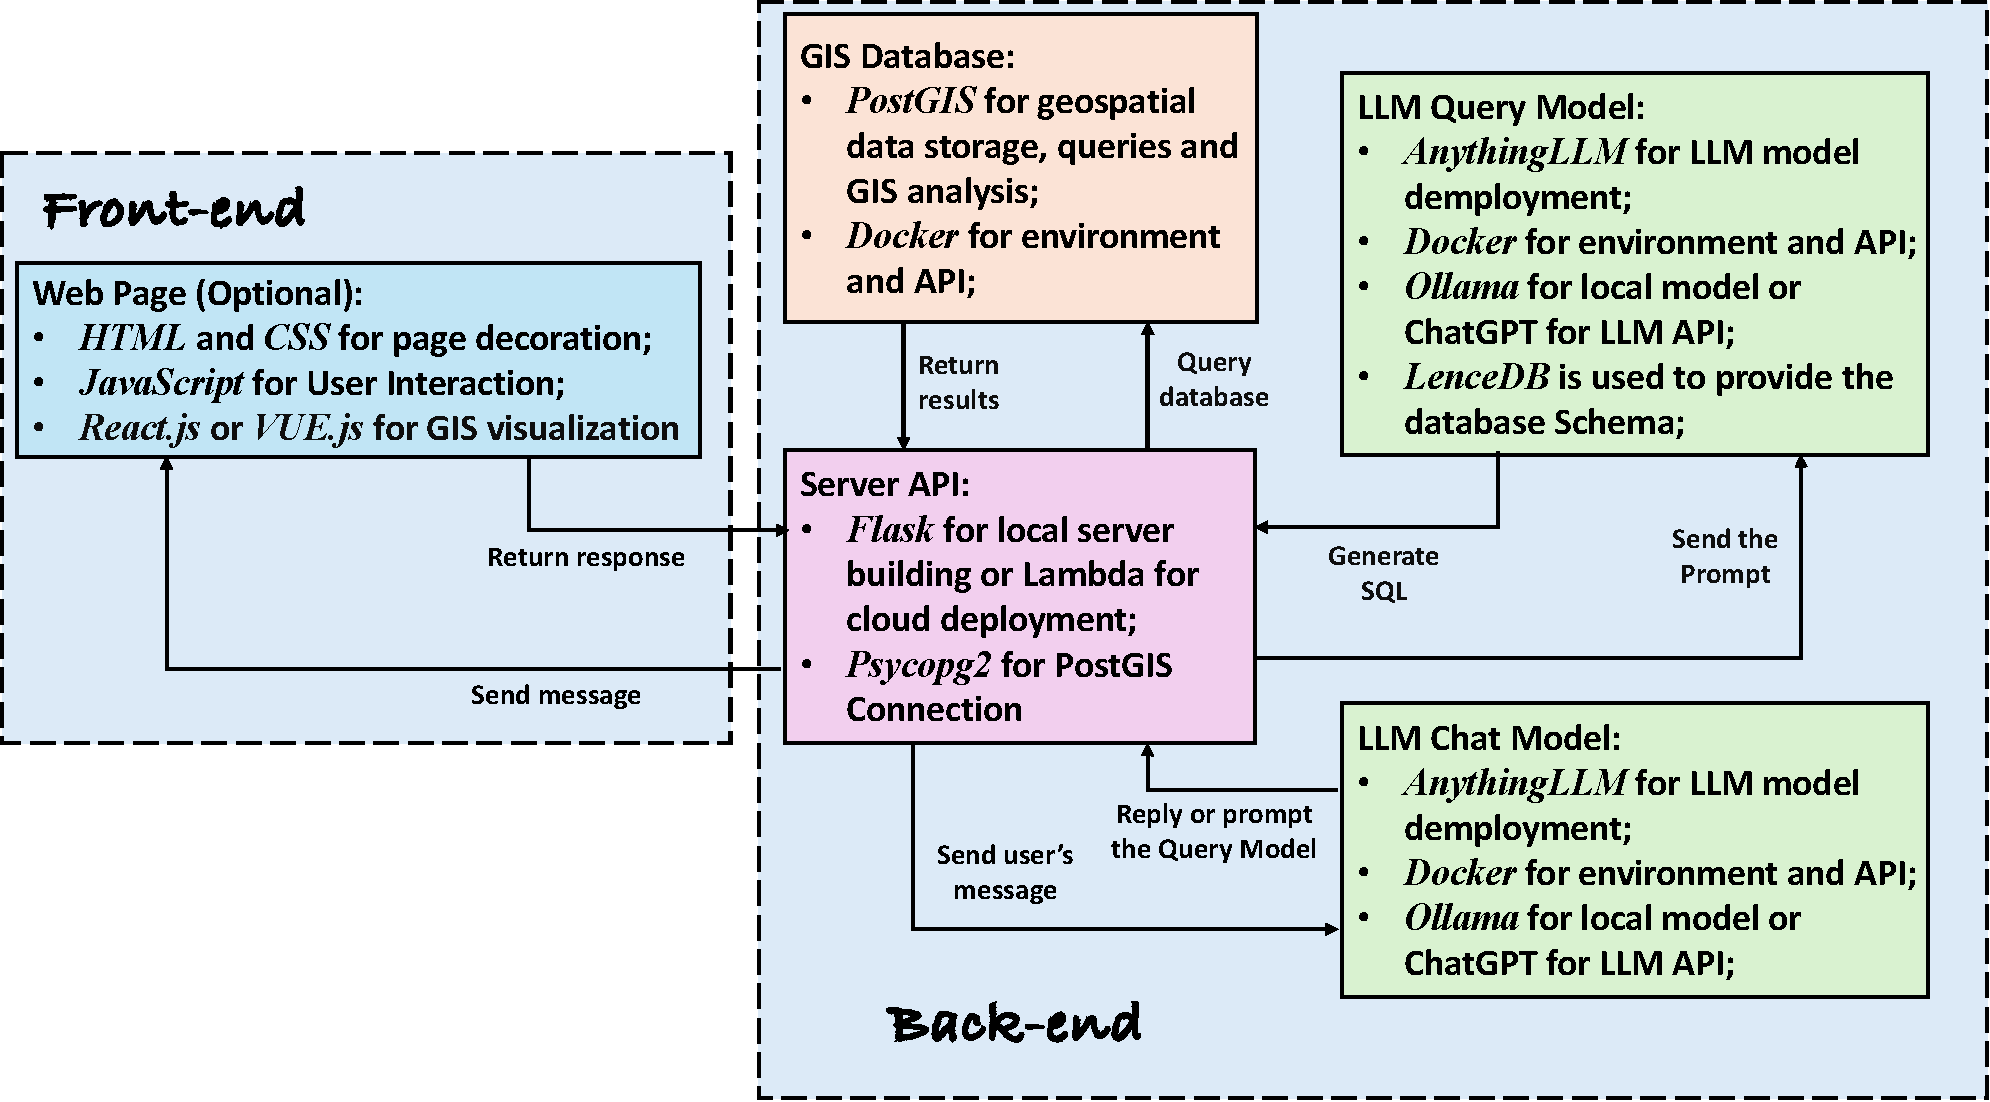
\includegraphics[width=\textwidth]{figs/techstack.pdf}
    \caption{Tech Stack Used}
    \label{fig:techstack}
\end{figure}

Need to note that the LLM Quey Model is only used to generate the optimized SQL statements, and the LLM Chat model is used to generate the natural language queries to respond the user's queries.

\subsection{Query Syntax Implementation}

In order to make the LLM generate the accuate SQL statements, we need to use the following steps:

\begin{enumerate}
    \item I store the schema of the database as csv files to nake the LLM know the structure of the database.
    \item I collect the fclass (The class of the object in the map. E,g., School, Restaurant, etc.) attributes in each table and store them in a csv file.
    \item I use the following senetances to prompt the  LLM to generate the SQL statements as shown in Appendix~\ref{app:llm_prompt}.
    \item Need to note that I will change the prompt sentence to make it the professional SQL generator. And I will use another prompt to build up the new LLM for chat with users.
\end{enumerate}


\subsection{Database Selection}
Because this project need many spatial computations, we use a spatial database called PostGIS. It is a powerful and flexible open-source database that supports a wide range of geospatial operations. It is also easy to use and has a large community of users.

\section{Planned Implementation}
The future implementation plan of our system is shown in Figure~\ref{fig:techstack}. Compared with the original plan, we have added the following changes:

\begin{enumerate}
    \item Firstly, we will build up 2 LLM model for this project. The first one is for the SQL query generation, and the second one is for the chat with users.
    \item Secondly,  in order to make the LLM understand the structure better and generate the SQL statements more accurately, we will reorganize the data with the fclass tagged in the database.
\end{enumerate}

\section{Project Status}
At the moment, we have finished the following steps:

\begin{enumerate}
    \item We finished the data collection from the OSM and the PostGIS database building. All data is imported and integrated into the database;
    \item We finished the environment setup for our LLM model. We have installed the necessary libraries and docker images;
    \item The prompted model can basically generate the SQL statements. But only few of them can get the correct result. We need to improve the prompted model and test it thoroughly.
\end{enumerate}

\section{Challenges Faced}
\begin{enumerate}
    \item The \textbf{BIGGEST} challange for this project is to make sure that the LLM model can understand the structure of the database and generate the SQL statements accurately. We need to test the system thoroughly and make sure that the generated SQL statements are correct.
    \item I am not very familar with the PostGIS and the OSM data. I need to learn more about them and how to use them.
    \item We may need to roorganize the database, which could be time-consuming;
    \item We are not sure that the interaction with two models and our server will be smooth. We need to test the system thoroughly;
\end{enumerate}

\section{Timeline}
Before the Final Presentation, we need to finish the following tasks:

\begin{enumerate}
    \item Reorganize the database with the fclass tagged in the database;
    \item Prompt the LLM to generate the SQL statements accurately.
    \item Build up the server for interactions.
    \item Build up the webpage for the chat with users if possible.
\end{enumerate}
% 参考文献部分
% \bibliography{references}  % 引用 BibTeX 文件 "references.bib"

\appendix

\section{Prompt information for LLM}
\label{app:llm_prompt}

{\ttfamily
You are ChatGIS, an AI assistant specializing in GIS data analysis and SQL query generation. Follow these strict rules:
\begin{enumerate}
    \item \textbf{Database Schema Inquiry}
    \begin{itemize}
        \item Answer questions about table structures, field names, and data types based on the provided database schema.
        \item Do not omit any fields—always list all available columns.
    \end{itemize}

    \item \textbf{SQL Query Generation}
    \begin{itemize}
        \item If asked for SQL, return only the exact query—no explanations unless explicitly requested.
        \item If the query cannot be answered directly from the files, return the SQL needed to extract the data.
        \item If the required data is missing, clearly state so.
    \end{itemize}

    \item \textbf{Strict Data Source Usage}
    \begin{itemize}
        \item Use only the uploaded files—do not assume or fabricate any data.
        \item If GIS-related data exists, provide it. Otherwise, generate an SQL query.
    \end{itemize}

    \item \textbf{Response Handling}
    \begin{itemize}
        \item If the question can be answered from the schema, provide the direct answer.
        \item Otherwise, return the SQL query to extract it.
        \item If the question is completely outside the provided data, suggest external sources only when necessary.
    \end{itemize}

    \item \textbf{Query Optimization Based on Data Availability}
    \begin{itemize}
        \item Before generating an SQL query, check \texttt{fclass\_counts.csv} to verify if relevant data exists.
    \end{itemize}

    \item \textbf{Schema-Specific Queries}
    \begin{itemize}
        \item All tables are under the california schema. Always include the schema name (california.) when referencing tables in SQL queries.
    \end{itemize}

    \item \textbf{Polygon Table Identification}
    \begin{itemize}
        \item Tables ending with "\_a" contain polygon geometries, while other versions of the same table may contain points or lines.
        \item Use only the polygon tables for area calculations.
    \end{itemize}
\end{enumerate}
}

\end{document}